\section{Cooperative attitude synchronization}
\label{sec:coop_att_syn}

Cooperative attitude synchronization is based on an undirected graph topology.
Theorem 3.1 \cite{5229134} is stated and proved to show that a proposed control law can drive the attitudes of all the agents to the reference attitude.
The distributed control law is given in equation \eqref{eq:coop_att_syn:ctrl_law} as follow.

For an agent $ i $, the control torque is 
\begin{subequations}
\label{eq:coop_att_syn:ctrl_law}
\begin{equation}
\dot{ \hat{x} }_{i} = \Gamma \hat{x}_{i} + \sum_{j=1}^{n} b_{ij}( \sigma_{i} - \sigma_{j} ) + k \sigma_{i},
\end{equation}
%\begin{equation}
%y_{i} = P \Gamma \hat{x}_{i} + P \sum_{j=1}^{n} b_{ij}( \sigma_{i} - \sigma_{j} ) + k P \sigma_{i},
%\end{equation}
\begin{equation}
\tau_{i} = - F^{T} ( \sigma_{i} ) \left[ \sum_{j=1}^{n} a_{ij}( \sigma_{i} - \sigma_{j} ) + a_{i(n+1)} (\sigma_{i} - \sigma_{c}^{r} ) + P \dot{ \hat{x} }_{i} \right].
\end{equation}
\end{subequations}
Let $ \hat{x} = [ \hat{x}^{T}_{1} , \cdots , \hat{x}^{T}_{n} ]^{T} $, $ \tau = [ \tau^{T}_{1} , \cdots \tau^{T}_{n} ]^{T}  $ and $ \sigma = [ \sigma^{T}_{1} , \cdots , \sigma^{T}_{n} ]^{T} $.
I can have the system dynamics as
\begin{subequations}
\label{eq:att_dyn_rig_bdy:mult_agt}
\begin{equation}
\label{eq:att_dyn_rig_bdy:mult_agt:a}
\dot{\sigma} = \bar{F}(\sigma) \omega,
\end{equation}
\begin{equation}
\label{eq:att_dyn_rig_bdy:mult_agt:b}
J \dot{\omega} = - \omega \times J \omega + \tau,
\end{equation}
where $ \bar{F}(\sigma) = diag( F(\sigma_{1}) , \cdots , F(\sigma_{n}) ) $.
\end{subequations}
Define $ J = diag( J_{1} , \cdots , J_{n} ) $ , $ T = L_{A} + diag[ a_{1(n+1)} , \cdots , a_{n(n+1)} ] $ and $ M = L_{B} + k I_{n} $, equation \eqref{eq:coop_att_syn:ctrl_law} can be expressed as \footnote{$ \otimes $ denotes Kronecker product.}
\begin{subequations}
\label{eq:coop_att_syn:ctrl_law:mult_agt}
\begin{equation}
\label{eq:coop_att_syn:ctrl_law:mult_agt:a}
\dot{\hat{x}} = ( I_{n} \otimes \Gamma ) \hat{x} + ( M \otimes I_{3} ) \sigma ,
\end{equation}
\begin{equation}
\label{eq:coop_att_syn:ctrl_law:mult_agt:b}
\tau = - \bar{F}^{T}(\sigma) [ ( T \otimes I_{3} )( \sigma - \mathbf{1}_{n} \otimes \sigma^{r}_{c} ) + ( I_{n} \otimes P ) \dot{ \hat{x} } ] .
\end{equation}
\end{subequations}

\subsection{Proof strategy}
\label{sec:coop_att_syn:proof}

The proposed Lyapunov function is 
\begin{equation}
V = \frac{1}{2} ( \sigma - \mathbf{1}_{n} \otimes \sigma^{r}_{c} )^{T} ( T \otimes I_{3} ) ( \sigma - \mathbf{1}_{n} \otimes \sigma^{r}_{c} ) + \frac{1}{2} \omega^{T} J \omega + \frac{1}{2} \dot{\hat{x}}^{T} ( M \otimes I _{3} )^{-1} ( I_{n} \otimes P ) \dot{\hat{x}}.
\end{equation}
There are several steps used in eliminating terms in $ \dot{V} $ to get the final form $ \dot{V} = - \frac{1}{2} \dot{\hat{x}}^{T} (M \otimes I_{3})^{-1} (I_{n} \otimes Q) \dot{\hat{x}} $.
\begin{itemize}
\item By $ \omega^{T}_{i} ( \omega_{i} \times J_{i} \omega_{i} ) = 0 $, I have
$ \omega^{T} ( \omega \times J \omega ) = \mathbf{0}_{n} $;
\item By $ M $ is symmetric (an undirected graph), $ M^{T} M^{-1} = I $
\item $ ( I_{n} \otimes \Gamma )^{T} ( M \otimes I_{3} )^{-1} ( I_{n} \otimes P ) = ( M \otimes I_{3} )^{-1} ( I_{n} \otimes \Gamma^{T} ) ( I_{n} \otimes P ) $;
\item $ \Gamma^{T} P + P \Gamma = - Q $.
\end{itemize}
When $ \dot{\hat{x}} $ converges to zero, it is derived that $ \sigma \equiv 0 $ and $ \sigma \equiv \mathbf{1}_{n} \otimes \sigma^{r}_{c} $.
By LaSalle's invariance principle, I can have $ \sigma_{i}(t) \rightarrow \sigma^{r}_{c} $ and $ \omega_{i} (t) \rightarrow 0 $ as $ t \rightarrow \infty $.

\subsection{How cooperative attitude synchronization works}
\label{sec:coop_att_syn:analysis}

As the transient performance can be ignored, I simplify the control law to figure out the terms help the system stability and the terms help the transient performance.

\subsubsection{Removing damping term $ ( M \otimes I_{3} ) \sigma $}
\label{sec:coop_att_syn:analysis:a}

There exists a damping term in updating $ \dot{\hat{{x}}} $, which facilitates the formation control. 
It helps the agents reduce the relative attitude difference with neighbors while moving towards the reference attitude $ \sigma^{r}_{c} $.
By removing the damping term $ ( M \otimes I_{3} ) \sigma $, the control law becomes
\begin{subequations}
\label{eq:coop_att_syn:ctrl_law:mult_agt:2}
\begin{equation}
\label{eq:coop_att_syn:ctrl_law:mult_agt:2:a}
\dot{\hat{x}} = ( I_{n} \otimes \Gamma ) \hat{x}  ,
\end{equation}
\begin{equation}
\label{eq:coop_att_syn:ctrl_law:mult_agt:2:b}
\tau = - \bar{F}^{T}(\sigma) [ ( T \otimes I_{3} )( \sigma - \mathbf{1}_{n} \otimes \sigma^{r}_{c} ) + ( I_{n} \otimes P ) \dot{ \hat{x} } ] .
\end{equation}
\end{subequations}
The proposed Lyapunov function is
\begin{subequations}
\label{eq:coop_att_sync:lyapunov_func:2}
\begin{equation}
V = \frac{1}{2} ( \sigma - \mathbf{1}_{n} \otimes \sigma^{r}_{c} )^{T} ( T \otimes I_{3} ) ( \sigma - \mathbf{1}_{n} \otimes \sigma^{r}_{c} ) + \frac{1}{2} \omega^{T} J \omega + \frac{1}{2} \dot{\hat{x}}^{T} ( I_{n} \otimes P ) \dot{\hat{x}},
\end{equation}
\begin{equation}
\dot{V} = - \frac{1}{2} \dot{\hat{x}}^{T} (I_{n} \otimes Q ) \dot{\hat{x}}.
\end{equation}
\end{subequations}
%By the definition of the damping term $ ( M \otimes I_{3} ) \sigma $, I can see that the damping term facilitates the formation control.
%It helps the agents keeping same/close attitudes and move together towards the reference attitude $ \sigma^{r}_{c} $.
In the same way, the stability can be proved.

\subsubsection{Replacing $ \dot{\hat{x}} $ with $ \dot{\sigma} $ }
\label{sec:coop_att_syn:analysis:b}

One of the contribution in Dr. Ren's paper \cite{5229134} is that there is no need of an angular velocity measurement as in previous work \cite{4777127}, which means that either $ \omega $ or $ \dot{ \sigma } $ is not needed in the control law. 
Thus I guess that the function of $ \hat{x} $ is used as an estimation of the $ \sigma $ or $ \phi $. 
$ \dot{ \hat{x} } $ can be replaced with $ \dot{ \sigma } $. 
I can have a modified control law
\begin{equation}
\label{eq:coop_att_syn:ctrl_law:mult_agt:3}
\tau = - \bar{F}^{T}(\sigma) [ ( T \otimes I_{3} )( \sigma - \mathbf{1}_{n} \otimes \sigma^{r}_{c} ) + K \dot{ \sigma } ] .
\end{equation}
The proposed Lyapunov function for stability is
\begin{subequations}
\label{eq:coop_att_sync:lyapunov_func:3}
\begin{equation}
V = \frac{1}{2} ( \sigma - \mathbf{1}_{n} \otimes \sigma^{r}_{c} )^{T} ( T \otimes I_{3} ) ( \sigma - \mathbf{1}_{n} \otimes \sigma^{r}_{c} ) + \frac{1}{2} \omega^{T} J \omega ,
\end{equation}
\begin{equation}
\dot{V} = - \dot{\sigma}^{T} K \dot{\sigma}.
\end{equation}
\end{subequations}
%Similarly, the stability can be proved.

\subsection{Simulation}
\label{sec:coop_att_syn:sims}

\begin{figure}
\centering
\begin{subfigure}{0.3\linewidth}
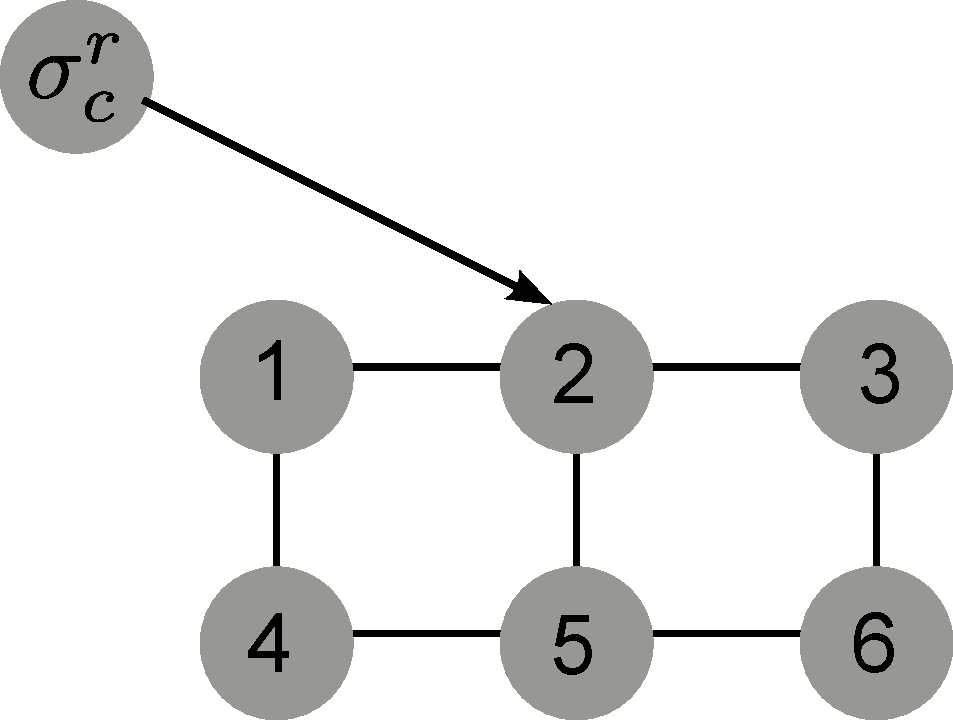
\includegraphics[width=\linewidth]{./images/csa_graph}
\caption{Undirected graph.}
\label{fig:cas:sims:graph}
\end{subfigure}
\begin{subfigure}{0.3\linewidth}
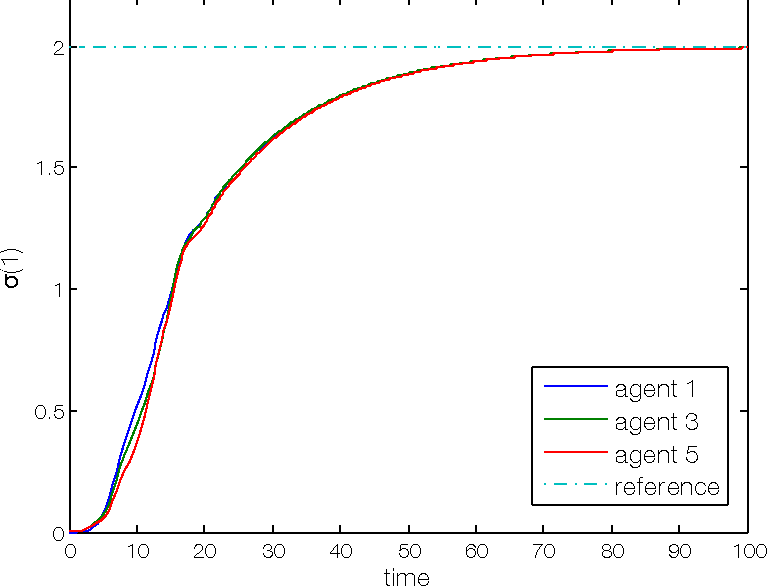
\includegraphics[width=\linewidth]{./images/cas_D1_1_3_5_dyn}
\caption{Dynamics of $ \sigma(1) $.}
\label{fig:cas:sims:dyn}
\end{subfigure}
\caption{Cooperative attitude synchronization.}
\label{fig:cas:sims}
\end{figure}

\begin{figure}
\centering
\begin{subfigure}{0.4\linewidth}
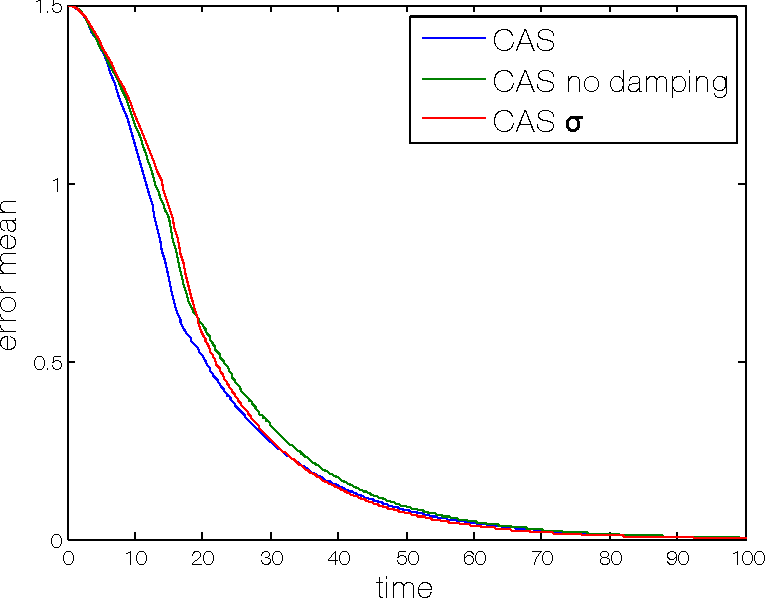
\includegraphics[width=\linewidth]{./images/cas_err_mean}
\caption{Mean - error.}
\label{fig:cas:sims1:mean}
\end{subfigure}
\begin{subfigure}{0.4\linewidth}
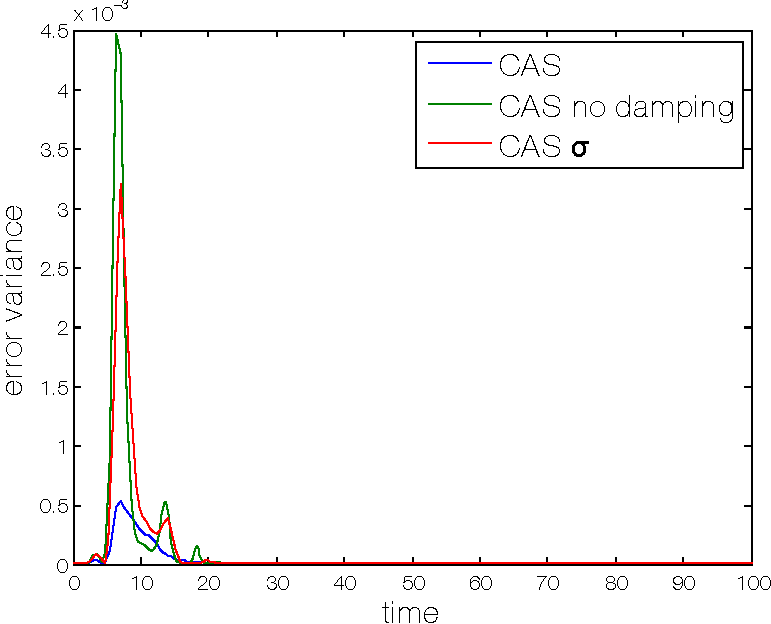
\includegraphics[width=\linewidth]{./images/cas_err_var}
\caption{Variance - error.}
\label{fig:cas:sims1:var}
\end{subfigure}
\caption{Comparison on different control laws.}
\label{fig:cas1:sims}
\end{figure}

\begin{figure}
\centering
\begin{subfigure}{0.4\linewidth}
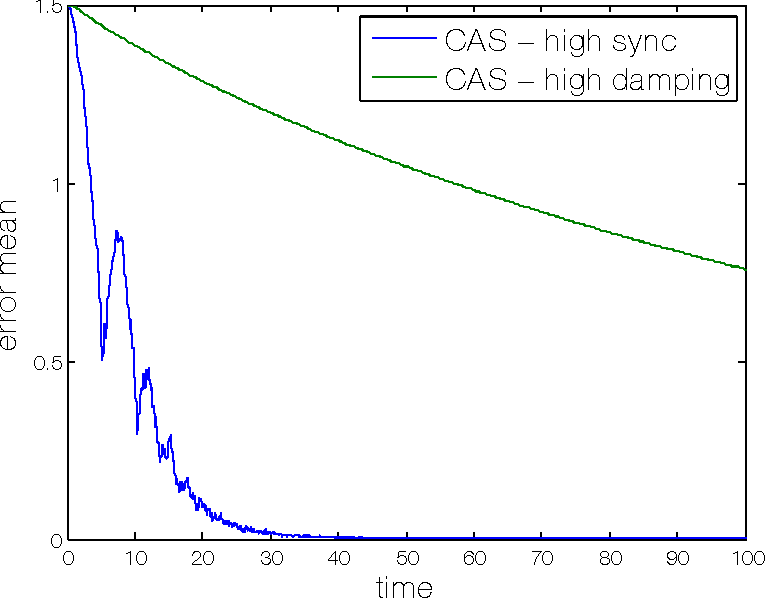
\includegraphics[width=\linewidth]{./images/cas_par_mean}
\caption{Mean - error.}
\label{fig:cas:sims2:mean}
\end{subfigure}
\begin{subfigure}{0.4\linewidth}
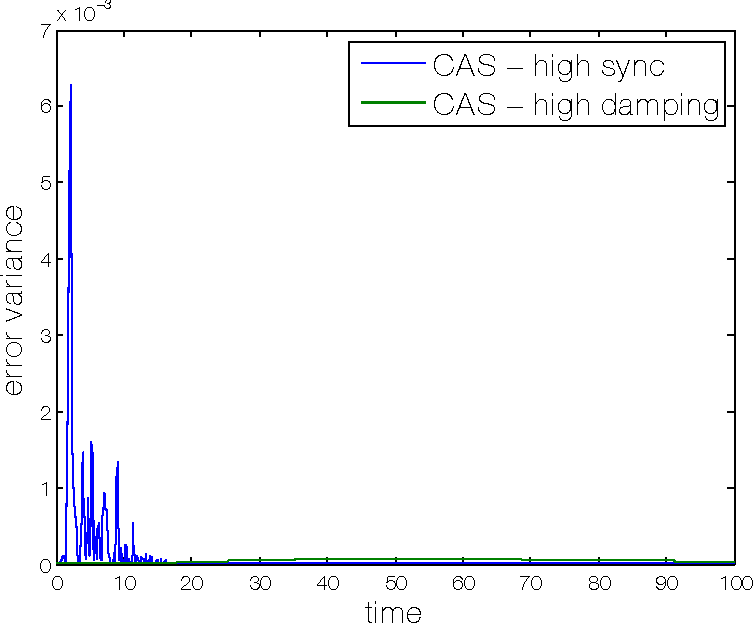
\includegraphics[width=\linewidth]{./images/cas_par_var}
\caption{Variance - error.}
\label{fig:cas:sims2:var}
\end{subfigure}
\caption{Comparison on different control parameters.}
\label{fig:cas:sims2}
\end{figure}

Simulations use the same parameters and network topology in Dr. Ren's paper \cite{5229134}.
The undirected graph is shown in Figure \ref{fig:cas:sims:graph}.
Figure \ref{fig:cas:sims:dyn} shows that all the agents converge to the reference attitude with a good formation.

The performances of different control laws are compared.
Figure \ref{fig:cas:sims1:mean} shows that they have same convergence rate.
However, without a damping term increases the variance of the agents' attitudes significantly, as shown in Figure \ref{fig:cas:sims1:var}.
Using $ \dot{\sigma_{i}} $ instead of $ \dot{x}_{i} $ can have better transiency on synchronization.
It is also tested that increasing the damping coefficient $ b_{ij} $ decreases the rate of converging the reference but keeps good group formation, which is shown in Figure \ref{fig:cas:sims2:mean} and Figure \ref{fig:cas:sims2:var}.
Increasing the synchronization coefficient $ a_{ij} $ leads to opposite results.
